%!TEX root = Main.tex
\section{Evaluation}
\label{sec:eval}

The goal of our evaluation is to answer the following questions: (1) How well does \auspice's distributed design meet its latency, cost, and availability goals compared to state-of-the-art alternatives? (2) Can \auspice\ serve the basis of a complete, end-to-end solution for mobility and enable novel communication abstractions? (3) How does \auspice's performance and cost compare against best-of-breed managed DNS services today?

%Our main goal is to quantify the benefits and costs of the choices in \auspice's distributed design---our main contribution---with respect to the subset of design goals  ($\S$\ref{sec:design_goals}) that are quantifiable, namely client-perceived latency benefit and provider-perceived update cost under high mobility. We use the implemented prototype to evaluate (1) \auspice's replication strategies against simple ones used by DNS providers today as well as DHT-based alternatives proposed in research, and (2) a deployment of \auspice\ against several commercial managed DNS providers in live operation. We use simulations to evaluate (3) the sensitivity of \auspice's benefits with respect to mobile workload parameters, and (4) the scalability of \auspice\ to regimes beyond those permitted by our testbeds. We do not attempt to evaluate \auspice's functional design goals---resilience to failures, consistency, extensibility, security---except to the extent that all experiments subsume the overhead of these features.

\eat{
The goals of our evaluation are to
(1) compare \auspice\ to alternative replica placement and redirection strategies including  DHT-based designs and simple baseline strategies, and 
(2) compare  \auspice\ to commercial managed DNS providers, which are currently the best available solution for authoritative DNS service for domain names. 
}
%authoritative name service providers, that offer a geo-replicated authoritative DNS service for domain names. 
%commercial authoritative name service providers, known as managed DNS providers. 
%state-of-the-art authoritative name service providers, known as  managed DNS providers.
% 

\eat{Our main results are:

%demonstrate TCP connection migration across networks using the MSocket library. The key results from our evaluation are:

\begin{itemize}
\item
\emph{Lookup latency:} \auspice\ provides 5.4$\times$-11.2$\times$ lower lookup latency than \codons, a DHT-based scheme which replicates names based on popularity.
\item
\emph{Capacity:} \auspice\  sustains  a request load that is 18$\times$ the maximum load sustained by a replicate-everywhere scheme, and is comparable to the maximum load sustained by DHT-based designs.
\item
\emph{Comparison to managed DNS:} \auspice\ achieves lookup latencies comparable to a leading managed DNS provider with only one-third the locations of name resolvers. \auspice\ provides a median update latency that is 1.1 sec to 24.7 sec lower than the median update latencies of managed DNS providers.
\item
\emph{Mid-session mobility:} MSocket library enables seamless end-user mobility by migrating a TCP connection from Wi-Fi to 4G in three round trip times.
\end{itemize}
}



\vspace{-0.1in}
\subsection{\auspice's distributed design}
We evaluate (1) the latency and cost benefits of \auspice's demand-aware placement compared to static placement schemes; and (2) the scalability of \auspice\ with the number of names over several orders of magnitude.
\subsubsection{Experiment setup}

\textbf{Testbeds:} We use a combination of geo-distributed testbeds (Amazon EC2 and Planetlab) and local clusters (a 100-node EC2 cluster or a 16-node departmental cluster) depending upon the goals of the experiment. The departmental cluster consists of 16 machines  (Xeon 5140, 4-core, 8 GB RAM)  and the EC2 instances are ``m3.xlarge" with 15GB RAM.


\textbf{Workload:} There is no real workload today of clients querying a name service in order to communicate with mobile devices frequently moving across different network addresses, both because such a name service does not exist and mobile devices do not have publicly visible IP addresses. So we conduct an evaluation using synthetic workloads for device names, but to avoid second-guessing future workload patterns, we conduct a comprehensive sensitivity analysis against all of the relevant parameters such as the read rate, write rate, popularity, and geo-locality of demand.

%A vexing evaluation  challenge is that we do not have a workload of clients querying a name service in order to communicate with mobile devices moving across different network addresses. There is no global name resolution infrastructure for mobile device names today and most mobile devices do not have publicly visible addresses, so no one queries for them.

The following are default experimental parameters (except for $\S$\ref{sec:sensitivity} on sensitivity analysis) for device names. The ratio of the total number of lookups across all devices to the total number of updates is 1:1, i.e., devices are queried for on average as often as they change addresses. The lookup rate of any single device name is uniformly distributed between 0.5 to 1.5 times the average lookup rate; the update rate is similarly distributed and drawn independently, so there is no correlation between the lookup and update rate of a name.


%\textbf{Workload:}  A real workload for a name service for mobile hosts does not exist today, as no global infrastructure supports name resolution for mobile hosts. Our evaluation uses a synthetic workload of names of mobile devices, called \emph{device names}, and we perform a sensitivity analysis of workload parameters in Section  \ref{sec:sensitivity}. Experiments other than  Section \ref{sec:sensitivity}  use following default parameters. Lookup and update rates of device names  follow a uniform distribution, with no correlation between the lookup rate and the update rate of a name. The ratio of total number of lookups to updates is 1:1.  

%are as follows.

%None of the characteristics of this workload, e.g., ratio of lookup to updates, distribution of popularity of names,  and geo-locality of requests, are known currently. Therefore, we evaluate performance for a range of workload parameters in Section  \ref{sec:sensitivity}.

%The default parameters of the workload for device names used in  

\begin{table}[t]
\centering
\small{
\begin{tabular}{c|c}
{\bf Workload parameter} & {\bf Value} \\ \hline
%Name servers & 80 %(100 in $\S$\ref{sec:optimal})  
%\\ \hline
%Local name servers	 & 80  %(100 in $\S$\ref{sec:optimal}) 
%\\ \hline
Fraction of (highly mobile) device names & 90\%  \\ \hline
Fraction of (mostly static) service names & 10\%   \\ \hline
\% of device name lookups   & 33.33\%  \\ \hline
\% of device name updates  & 33.33\% \\ \hline
\% of service name lookups   & 33.33\%  \\ \hline
\% of service name updates  & 0.01\% \\ \hline
Geo-locality: [devices, services] & [0.75, 0.8]  \\ \hline
\end{tabular}
}
\caption{Default experiment parameters (except $\S$\ref{sec:sensitivity}).}
\vspace{-0.15in}
\label{tab:setup}
\end{table}


How requests are geographically distributed is clearly important for evaluating a replica placement scheme.  We define the {\em geo-locality} of a name as the fraction of requests from top-10\% of regions where the name is most popular. This parameter ranges from 0.1 (least locality) to 1 (high locality). For a device name with  geo-locality of $g$,  a fraction $g$ of the requests are assumed to originate from N=10\% of the local name servers, the first of which is picked randomly and rest N-1 are the local name servers geographically closest to it. How do we pick a reasonable $g$? With admittedly little basis, we pick $g=0.75$ for device names, i.e., the top-10\% of regions in the world will account for 75\% of requests to device names, an assumption not altogether unreasonable given that communication and content access today exhibits a high country-level locality \cite{twitter-www, locality-conext}.


%For this, we turn to the geo-locality exhibited today by the top 100,000 websites, which we calculated using the Alexa dataset \cite{alexa} to be 0.8. So, with little else to go by, we pick $g=0.75$ for device names, i.e., the top-10\% of regions in the world will account for 75\% of requests to device names, an assumption not altogether unreasonable given that communication and content access today exhibits a high country-level locality \cite{remove-if-no-citation}.

%randomly chosen local name server and (N - 1) local name servers that are geographically closest to it (N = 10\% of local name servers);  remaining requests are generated from random locations. 

%We have calculated that the average geo-locality for top 100K websites  in the Alexa dataset is 80\% \cite{alexa}. Therefore, in most experiments, we use workloads where the geo-locality of device names is 75\%. 

%To select the geo-locality parameter of device names, we analyze the locality in the request patterns for today's web services from the Alexa dataset \cite{alexa}. 

In addition to device names, {\em service names} constitute a small fraction (10\%) of names in the workload and are intended to capture web services like today with low mobility. Their lookup rate (or popularity) distribution and geo-distribution are used directly from the Alexa dataset\footnote{Note that we do not rely on Alexa at all for mobile device names.} \cite{alexa}. Using this dataset, we calculated the geo-locality exhibited by the top 100,000 websites to be 0.8. Updates for service names are a tiny fraction ($0.01\%$) of lookups, as web services can be expected to be queried much more often than they are moved around. The lookup rate of service names is a third of the total number of requests (same as the lookup or update rates of device names).

%Overall, service name lookups, device name lookups, device name updates each receive about a third each of the total number of requests, 

Table \ref{tab:setup} summarizes the default workload parameters.

%\auspice\ would provide name resolution both for highly mobile hosts and for hosts with low mobility,  e.g., web services. Our workload contains a small fraction (9\%)  of names of web services, called \emph{service names}.  The distribution of request rates and and geo-distribution of requests for service names are generated based on the Alexa dataset \cite{alexa}. In experiments with 1K (10K) service names, we use statistics for top-1K (top-10K) websites  to generate our workload.   Updates for service names are a tiny fraction ($0.01\%$) of lookups, which is representative of the infrequent mobility of these web services. 


%Requests for service names are generated based on the Alexa dataset \cite{alexa}, which reports the relative popularity of top Internet websites and the geo-distribution of their popularity at city-level granularity. 
%Each city is mapped to the geographically closest local name server in our experiment.
%  Updates for service names are a tiny fraction ($0.01\%$) of lookups as web services are today's web services exhibit to have much lower mobility. 

%, as our measurement of name records of these websites shows that their addresses change slowly (on the order of weeks). 

%We empirically evaluate the performance of \auspice\ for a  range of workload parameters for device names.  Our synthetic workload for device names has following parameters:  (1) ratio of device names to service names, (2) ratio of total number of lookups to total number of updates for device names,  (3) geo-locality of requests for device names. Geo-locality is quantitatively defined using a parameter $p$, where higher values of $p$ imply weaker geo-locality. Specifically, a  geo-locality of $p$ $(0 \leq p \leq 1)$ means that a fraction $p$ of all requests for a name come from randomly chosen locations and remaining requests are generated from $X$ local name servers which are geographically close to each other;  $X$ is a uniformly distributed integer between 1 to  (5\% of number of local name servers). 

\eat{

% older workload section.
Our workload consists of  address lookups and updates from geo-distributed clients. The workload has two types of names: (1) \emph{Device names} are name records for mobile devices. (2) \emph{Service names} correspond to name records for web services, e.g., amazon.com.  This classification is used only for workload generation and none of the schemes distinguish between the two types of names.


Lookups for service names are generated based on the Alexa dataset \cite{alexa}, which reports the relative popularity of top Internet websites and the geo-distribution of their popularity at city-level granularity. Each city is mapped to the geographically closest local name server in our experiment.
In experiments with 1K (10K) service names, we use top-1K (top-10K) alexa websites information to generate our workload.  Updates for service names are a tiny fraction ($0.01\%$) of lookups. 
This is because our measurement of name records of these websites shows that their addresses change slowly (on the order of weeks). The local name servers sending the updates are chosen randomly for each name.



We have generated a synthetic workload for device names as it is difficult to predict the characteristics of a future workload for device names. We empirically evaluate the performance of \auspice\ for a  range of workload parameters for device names.  Our synthetic workload for device names has following parameters:  (1) ratio of device names to service names, (2) ratio of total number of lookups to total number of updates for device names,  (3) geo-locality of requests for device names. Geo-locality is quantitatively defined using a parameter $p$, where higher values of $p$ imply weaker geo-locality. Specifically, a  geo-locality of $p$ $(0 \leq p \leq 1)$ means that a fraction $p$ of all requests for a name come from randomly chosen locations and remaining requests are generated from $X$ local name servers which are geographically close to each other;  $X$ is a uniformly distributed integer between 1 to  (5\% of number of local name servers). 
}
  

%quantitatively defined using a parameter. 
%90\% of lookups are generated from $X$ local name servers which are geographically close to each other and remaining 10\% lookups are generated from randomly chosen local name servers.  All updates are generated from one of the $X$ local name servers. 
%$X$ is a uniformly distributed integer between 1 to  (5\% of number of local name servers). 


%Geo-locality is defined as follows: 

%Our workload has a comparable number of lookups and updates, and has a strong geo-locality. 
%In most experiments, the total number of lookups is equal to the total number of lookups.
%In most of the experiments, total number of updates for device names is equal to the total number of lookups for them. 
%The geo-distribution of lookups for a device name is as follows.  90\% of lookups are generated from $X$ local name servers which are geographically close to each other and remaining 10\% lookups are generated from randomly chosen local name servers.  All updates are generated from one of the $X$ local name servers. 



%****lookups and updates****


%(1) lookup-to-update ratio. 
%(2) geo-locality. 



%Table \ref{tab:setup} lists the parameters for experiments in Section \ref{sec:lookup} - \ref{sec:updatelatency}. 
%We present a sensitivity analysis of these workload parameters in Section \ref{sec:sensitivity}. 



%\begin{figure*}
%\subfigure[Lookup latencies.]{\label{fig:querylatencycdf}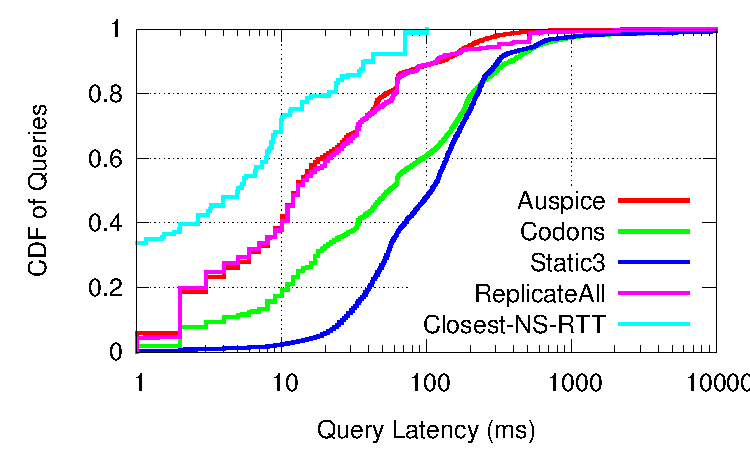
\includegraphics[scale=0.45]{auspice/graph/system-exp/cdf-comparison.pdf}}
%\subfigure[Median lookup latencies for names.]{\label{fig:namesquerymediancdf}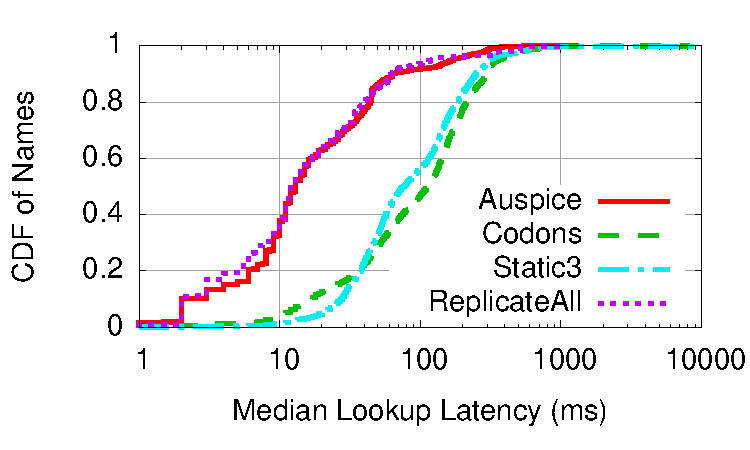
\includegraphics[scale=0.45]{auspice/graph/system-exp/cdf-names-median.pdf}}
%\subfigure[Update cost of names.]{\label{fig:updatebw}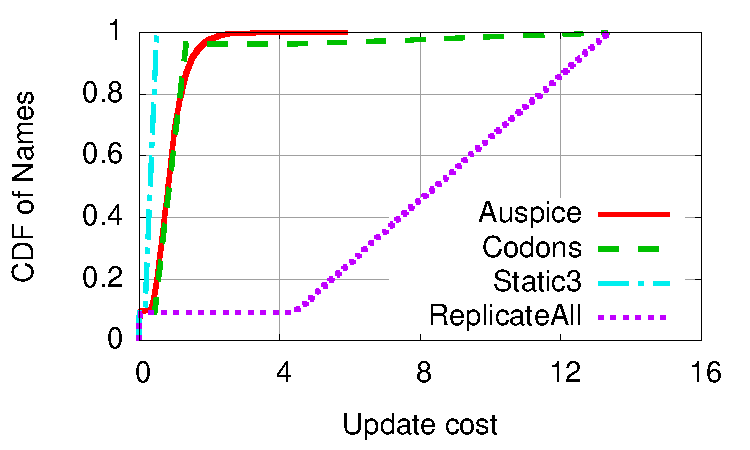
\includegraphics[scale=0.45]{auspice/graph/system-exp/cdf-update-cost.pdf}}
%\vspace{-0.1in}
%\caption{\auspice's lookup latency is nearly equal to \replicateall, yet its median update cost is 10$\times$ less. Locality-unaware schemes, \staticthree\ \& \codons, result in up to 6$\times$ higher median latencies than \auspice.}
%\vspace{-0.1in}
%\label{fig:lookupupdate}
%\end{figure*}


\eat{
\vsp
\subsubsection{Geographic locality}

To assess the extent of geo-locality in DNS names today, we conduct an analysis of Alexa's dataset \cite{alexa}. We measure geo-locality by dividing the world's land area into 1000 grids and counting access from any point in a grid as access from that grid. 20\% websites are accessed in less than 10\% of the geo areas for the top 100 and 1K sites and the percentage value goes up to 70\% for the top 100K sites.  Further, we find that for two of the top 10 sites (baidu.com and qq.com), 95\% of the demand comes from a single country, China, while for a third, amazon.com, 75\% of the demand originates from the US alone. This observed high locality of even popular names today suggests that locality-aware replica placement can significantly reduce lookup latency at a low update cost. We expect traffic originating from or destined to mobile names (both mobile-to-mobile as well as mobile-cloud traffic) to exhibit even more locality, especially with the increasing growth of location-aware mobile services and because most of a user's personal contacts are likely to be from small number of geo-regions.
}
%Replicating name records in locality-aware manner minimizes request latencies as well as update costs. 
%If request patterns show geo-locality, placing a small number of resolvers in a locality-aware manner can achieve low request latencies at a low cost. To assess the extent of geo-locality in DNS names today, we conduct an analysis of Alexa's dataset \cite{alexa}  that provides statistics about page views (refer to $\S$\ref{sec:eval} for more details of this dataset) that we expect to be correlated with the number of name lookups for the corresponding domain name.

%Our analysis of of geo-distribution of today's websites' traffic suggests that request patterns for their name records  show a high degree of geo-locality\tbd{Do you have a breakdown by grids of fixed size? Countries can vary greatly in size. Also, are google and facebook accessed in just 40 countries? This seems very likely wrong.}. We argue that name records for mobile hosts are likely to show even stronger geo-locality patterns, thereby making the case for a locality-aware placement of resolvers\tbd{On what basis are you arguing? Do you have a reference or a justification?}.

%Our design is motivated in part by two key features of the workload that the naming service is expected to handle: high update rates of name records, and geo-locality of distribution of requests.  A mobile host rapidly changes the set of networks it is connected to and thus requires frequent updates to its name record. 
 
\eat{
\begin{table}[t]
\centering
\small{
\begin{tabular}{ l | c | c}
\hline
rank \& site & \# countries & country most accessed\\
  & accessing  & \& traffic percentage\\
\hline
\hline
1, google.com & 36 & US \ 37.3\% \\ 
\hline
2, facebook.com & 40 & US \ 19.6\% \\
\hline
3, youtube.com & 39 & US \ 19.1\% \\
\hline
4, yahoo.com & 31 & US \ 32.8\% \\
\hline
\rowcolor[gray]{0.9} 5, baidu.com & 5 & CN \ 96.8\% \\
\hline
6, wikipedia.org & 34 & US \ 19.9\% \\
\hline
7, live.com & 33 & US \ 15.3\%\\
\hline
\rowcolor[gray]{0.9} 8, amazon.com & 19 & US \ 74.9\%\\
\hline
\rowcolor[gray]{0.9} 9, qq.com & 5 & CN \ 95.5\%\\
\hline
10, twitter.com & 31 & US \ 26.4\%\\
 \hline
\end{tabular}
}
\caption{Locality in top 10 sites: two sites baidu.com and qq.com have 95\% traffic coming from a single country.}
\vspace{-0.1in}
\label{tab:top10web}
\end{table}
}



\begin{figure*}[ht]
\subfigure[Lookup latencies (load = 0.3)]{\label{fig:namesquerymediancdf}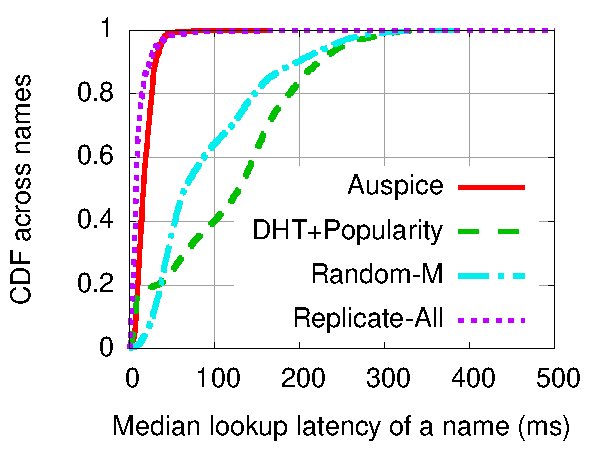
\includegraphics[scale=0.55]{auspice/graph/newgraphs/lookup-latency-cdf.pdf}}
\subfigure[Lookup latency-vs-load]{\label{fig:load}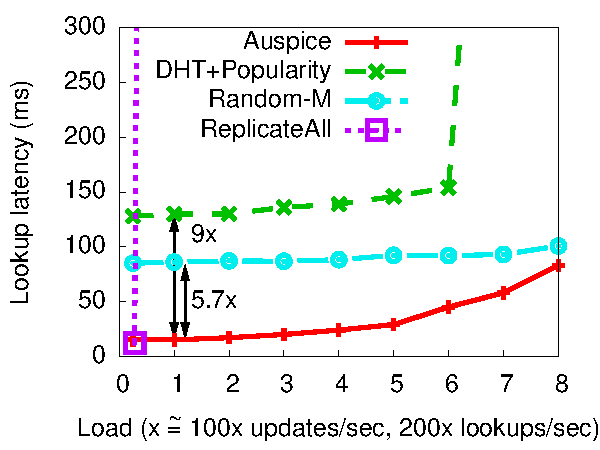
\includegraphics[scale=0.57]{auspice/graph/newgraphs/load-latency.pdf}}
\subfigure[Update cost-vs-load]{\label{fig:loadupdatecost}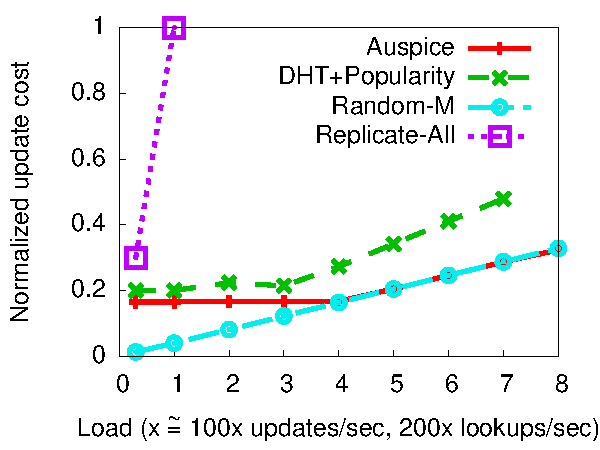
\includegraphics[scale=0.57]{auspice/graph/newgraphs/load-updatecost.pdf}}
%\subfigure[Update cost]{\label{fig:updatebw}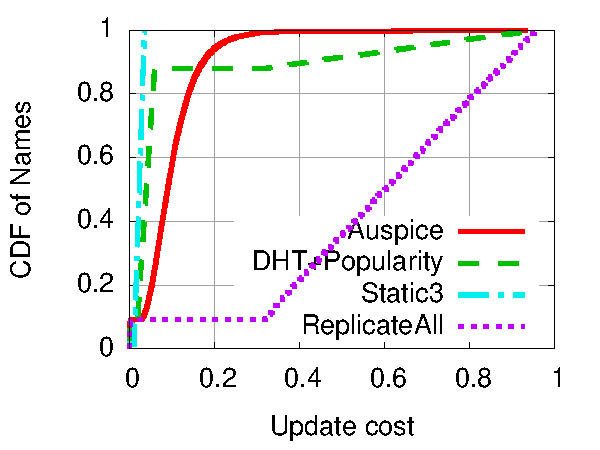
\includegraphics[scale=0.55]{auspice/graph/newgraphs/cdf-update-cost.pdf}}
\vspace{-0.15in}
\caption{[System] \auspice\ gives up to 5.7$\times$ to $9\times$ lower latencies over \staticthree\ and \codons\ respectively (Figure \ref{fig:load} at load=1). A load of 1 corresponds to 200 lookups/sec and 100 updates/sec. \replicateall\ peaks out at a load of 0.3 as it makes 80 replicas for each name while \auspice\ can sustain a request load of up to 8 as it chooses between 3 and 80 replicas per name.}
\vspace{-0.15in}
\label{fig:lookupupdate}
\end{figure*}


 
%We analyze geo-locality of today's websites using Alexa TopSites dataset  \cite{alexa}, which provides ranking of today's top websites, and geo-distribution  of  each website's requests. These statistics are based on page views for each website, but we expect the number of name record requests for a website to be proportional  (or positively correlated) to its page views in a geographic region. 


%Figure \ref{fig:localityweb} shows the geo-locality in website popularity: it plots the percentage of websites that are accessed in different fraction of geographical land areas\footnote{To measure it, we divide the world's land area into 1000 grids and count access from any point in a grid as access from that grid. }. 20\% websites are accessed in less than 10\% of the geo areas for the top 100 and 1K sites and the percentage value goes up to 70\% for the top 100K sites.  Further, we find that for two of the top 10 sites (baidu.com and qq.com), 95\% of the demand comes from a single country, China, while for a third, amazon.com, 75\% of the demand originates from the US alone. This observed high locality of even popular names today suggests that locality-aware replica placement can significantly reduce lookup latency at a low update cost. We expect traffic originating from or destined to mobile names to exhibit even more locality, especially with the increasing growth of location-aware mobile services. Thus, locality-awareness is an important design goal in \auspice.


{\textbf{Replication schemes compared:}}
%\label{sec:schemes}
\textbf{\auspice} uses the replication strategy with default parameter values as described in $\S$\ref{sec:design}. %We set the replication control parameter ($\beta$)  to ensure that the utilization of the servers remains below  70\% (refer to Equation \ref{eq:mu}). 
We compare against the following other schemes. \textbf{\staticthree} replicates each name at three random locations, and \textbf{\replicateall} replicates all names at all locations. \textbf{\codons} replicates name records using distributed hashing with replication similar in spirit to Codons\cite{codons-paper}. The number of replicas is chosen based on the popularity ranking of a name and  the location of replicas is decided by consistent hashing. The average hop count in Codons's underlying Beehive \cite{beehive} algorithm is set so that it creates the same average number of replicas as \auspice\ for a fair comparison. All schemes direct a lookup to the closest available replica after the first request.

%In our implementation, each request is directly sent to the replica  that would have received this request if Pastry  routing were followed, i.e., the latency we report would be smaller than the actual latency in \codons.   We set the Zipf exponent to be $0.63$ calculated based on our workload. The average hop count is set so that \codons\ creates the same number of replicas as  \auspice\ for a fair comparison.


\eat{\begin{figure*}[t]
\begin{minipage}[b]{0.3\linewidth}
\centering
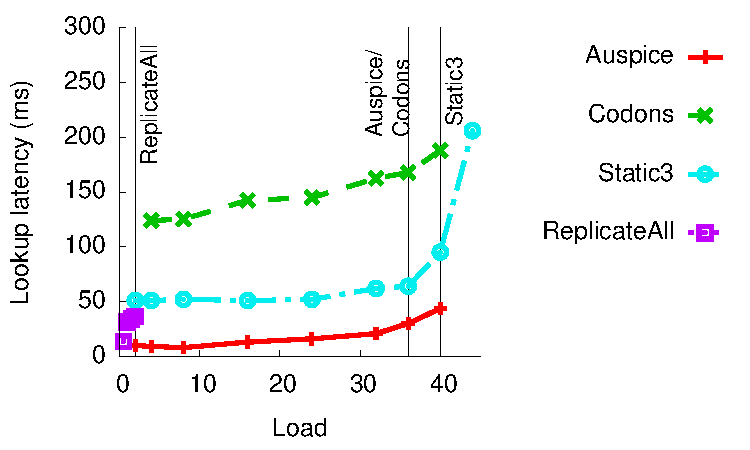
\includegraphics[scale=0.55]{auspice/graph/system-exp/system-load.pdf}
\caption{[Cluster] \auspice\ has lower latencies over \staticthree\ and \codons\ over a wide range of loads and can sustain loads up to 36. \replicateall\ saturates capacity at load of 2. ***Carefully word the captions.***}
\label{fig:load}
\end{minipage}
\hspace{0.5cm}
\begin{minipage}[b]{0.3\linewidth}
\centering
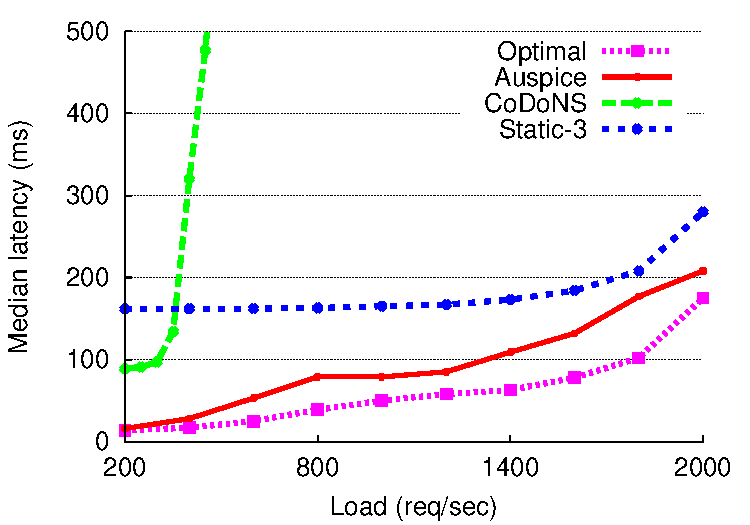
\includegraphics[scale=0.4]{auspice/graph/medianlatencyVSload_optimal.pdf}
\caption{[Simulator] \auspice's  latency is between 1.14$\times$ and 2.12$\times$  of \optimal. *** boxes the same size.***}
\label{fig:optimal}
\end{minipage}
\hspace{0.5cm}
\begin{minipage}[b]{0.3\linewidth}
\centering
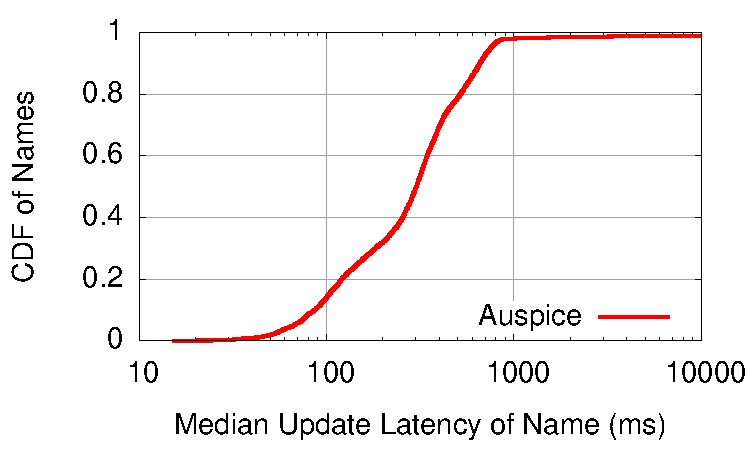
\includegraphics[scale=0.45]{auspice/graph/system-exp/cdf-names-median-update.pdf}
\caption{Address update latency of \auspice\ is comparable to other schemes. The high latencies for \replicateall\ are because of insufficient upload capacity on PlanetLab.}
\label{fig:udpates}
\end{minipage}
\vspace{-0.15in}
\end{figure*}
}

%\eat{
%\begin{figure*}[t]
%\begin{minipage}[b]{0.6\linewidth}
%\centering
%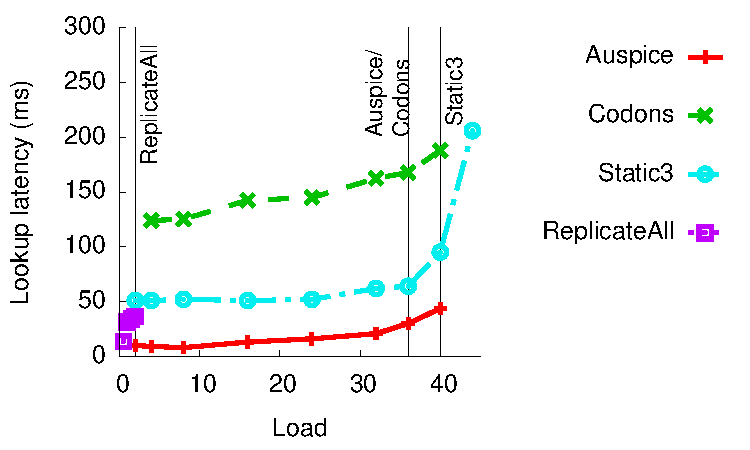
\includegraphics[scale=0.4]{auspice/graph/system-exp/system-load.pdf}
%\caption{[Cluster] \auspice\ has lower latencies over \staticthree\ and \codons\ over a wide range of loads and can sustain loads up to 36. \replicateall\ saturates capacity at load of 2. ***Carefully word the captions.***}
%\label{fig:load}
%\end{minipage}
%\hspace{0.5cm}
%\begin{minipage}[b]{0.3\linewidth}
%\centering
%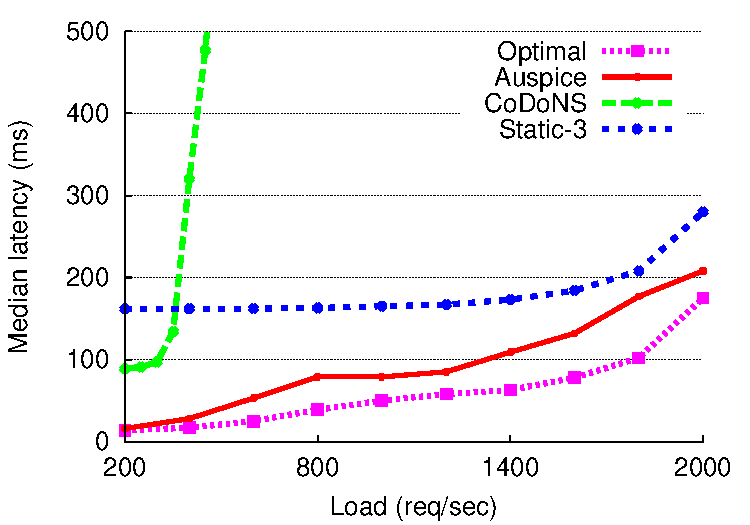
\includegraphics[scale=0.4]{auspice/graph/medianlatencyVSload_optimal.pdf}
%\caption{[Simulator] \auspice's  latency is between 1.14$\times$ and 2.12$\times$  of \optimal. *** boxes the same size.***}
%\label{fig:optimal}
%\end{minipage}
%\hspace{0.5cm}
%\begin{minipage}[b]{0.3\linewidth}
%\centering
%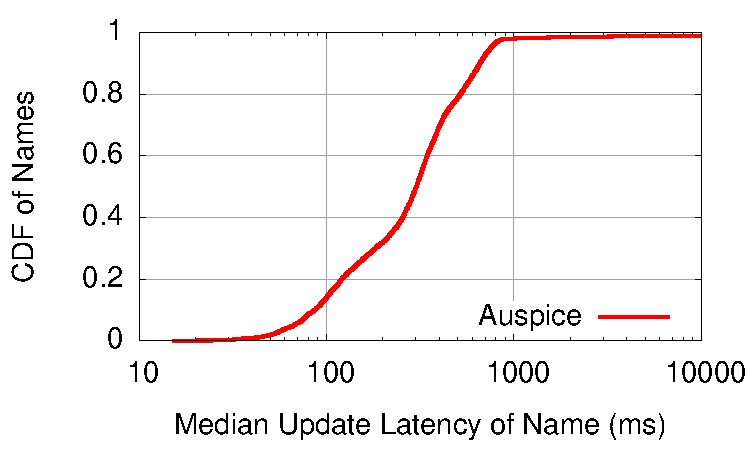
\includegraphics[scale=0.45]{auspice/graph/system-exp/cdf-names-median-update.pdf}
%\caption{Address update latency of \auspice\ is comparable to other schemes. The high latencies for \replicateall\ are because of insufficient upload capacity on PlanetLab.}
%\label{fig:udpates}
%\end{minipage}
%\vspace{-0.15in}
%\end{figure*}
%}

\vsp
\subsection{Comparison of replication schemes}
\label{sec:comparison}

We conduct experiments in this subsection on the 16-machine departmental cluster, wherein each machine hosts 10 instances of either nameservers or local nameservers so as to emulate an 80-nameserver \auspice\ deployment. We instrument the instances so as to emulate wide-area latencies between any two instances that correspond to 160 randomly chosen Planetlab nodes. We choose emulation instead of a geo-distributed testbed in this experiment in order to obtain reproducible results while stress-testing the load-vs.-response time scaling behavior of various schemes given identical resources.

%We present three experiments comparing schemes based on their lookup latency at varying request loads. First, we compare the lookup latency and update cost of schemes at a low request load. Second, we analyze the load-vs-lookup latency behavior of schemes and compare the capacity achieved by them. Third, we compare  \auspice\ to the \optimal\ strategy. 
\vsp
\subsubsection{Lookup latency and update cost}
\label{sec:lookup}
\label{sec:lowload}


%\auspice's lookup latency is nearly equal to \replicateall, yet its mean update cost is more than 5$\times$ smaller. \codons, a DHT-based scheme, results in up to 9$\times$ higher median latencies than \auspice.

%\begin{figure}[ht]
%\centering
%\subfigure[Lookup latency]{\label{fig:load}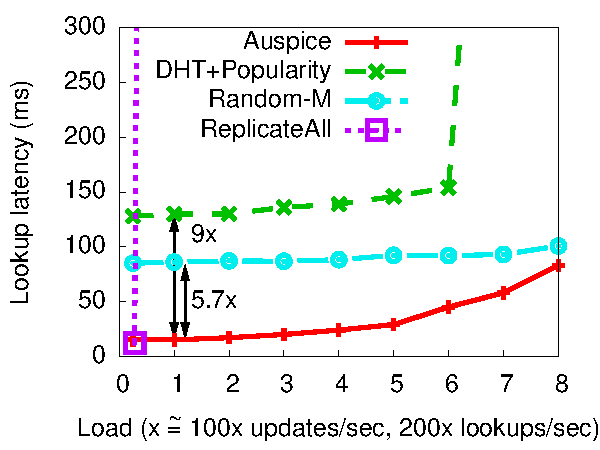
\includegraphics[scale=0.57]{auspice/graph/newgraphs/load-latency.pdf}}
%\subfigure[Update cost]{\label{fig:loadupdatecost}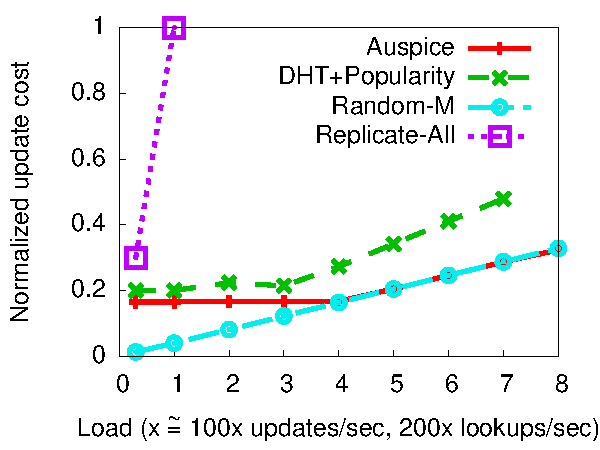
\includegraphics[scale=0.57]{auspice/graph/newgraphs/load-updatecost.pdf}}
%\caption{[Cluster] \auspice\ shows 2.2$\times$ to $9\times$ lower latencies over \staticthree\ and \codons\ over a wide rage of loads (0.3 - 6).  \auspice\ can sustain 23$\times$ higher loads than  \replicateall\ due to its lower update costs.}
%\vspace{-0.15in}
%\end{figure}


%

%\subsubsection{Lookup latency \& update cost  at low load}
%\label{sec:lowload}
%\begin{figure}[ht]
%\vspace{-0.05in}
%\subfigure[Median lookup latencies for names.]{\label{fig:namesquerymediancdf}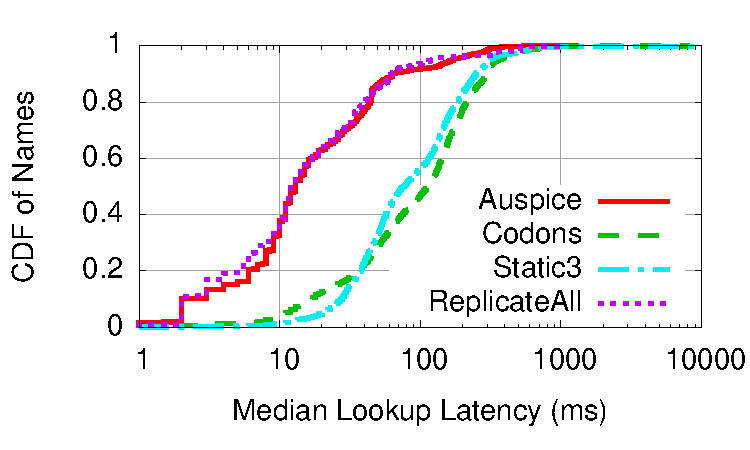
\includegraphics[scale=0.55]{auspice/graph/system-exp/cdf-names-median.pdf}}
%\subfigure[Update cost of names.]{\label{fig:updatebw}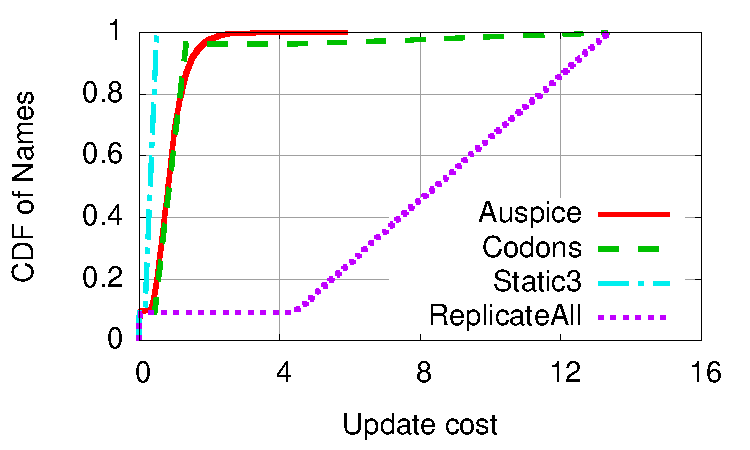
\includegraphics[scale=0.55]{auspice/graph/system-exp/cdf-update-cost.pdf}}
%\vspace{-0.1in}
%\caption{\auspice's lookup latency is nearly equal to \replicateall, yet its median update cost is 10$\times$ less. Locality-unaware schemes, \staticthree\ \& \codons, result in up to 6$\times$ higher median latencies than \auspice.}
%\vspace{-0.15in}
%\label{fig:lookupupdate}
%\end{figure}

%This experiment compares lookup latency of schemes at a low request load. We conduct this experiment with a workload of 400K lookups and 200K updates. The experiment runs for 15 minutes for every scheme. 
%Both \auspice\ and \codons\ pre-compute the placement at the start of the experiment based on prior knowledge of the workload, and retain the set of active replicas during the experiment. 


How well does \auspice\ use available resources for replicating name records? To evaluate this, we compare the lookup latency of schemes across varying load levels. A machine running 10 name servers receives on average 2000 lookups/sec and 1000 updates/sec at a load = 1. For each scheme, load is increased  until  2\% of requests fail, where a failed request means no response is received within 10 sec. The experiment runs for 10 mins for each scheme and load level. To measure steady-state behavior, both \auspice\ and \codons\ pre-compute the placement at the start of the experiment based on prior knowledge of the workload.%and retain the set of active replicas during the experiment. 

Figure \ref{fig:namesquerymediancdf} shows the distribution of median lookup latency across names at the smallest load level (load = 0.3).  Figure \ref{fig:load} shows load-vs-lookup latency curve for schemes, where ``lookup latency" refers to the mean of the median lookup latencies of names. Figure \ref{fig:loadupdatecost} shows the corresponding mean of the distribution of update cost across names at varying loads; the update cost for a name is the number of replicas times the update rate of that name.


{\em{\replicateall}}   gives low lookup latencies at the smallest load level, but generates a very high update cost and can sustain a request load of at most 0.3. This is further supported by  Figure \ref{fig:loadupdatecost} that shows that the update cost for \replicateall\ at load = 0.4 is more than the update cost of \auspice\  at load = 8. In theory, \auspice\ can have a capacity advantage of up to N/M over \replicateall, where N is the total number of name servers and M is the minimum of replicas \auspice\ must make for ensuring fault tolerance (reps. 80 and 3 here).

%It can sustain the cost of updating all replicas because the request load is very small.

{\em{\staticthree}} can sustain a high request load (Fig. \ref{fig:load}) due to its low update costs, but its lookup latencies are higher as it only creates 3 replicas randomly. %In theory, at low loads, \auspice\ can incur up to N/3 times more replication cost than \staticthree\ (but gain latency benefits), while at high loads, \auspice\ incurs an update cost comparable to \staticthree\ with a modest latency benefit because of better replica placement.

{\em{\auspice}}  gives up to 5.7$\times$ to $9\times$ lower latencies over \staticthree\ and \codons\ respectively (Figure \ref{fig:load}, load = 1). This is because it places a fraction of the replicas close to pockets of high demand unlike the other two.  At low to moderate loads, servers have excess capacity than the minimum needed for fault tolerance, so \auspice\ creates as many replicas as it can without exceeding the threshold utilization level (Equation \ref{eq:mu}), thereby  achieving very small latencies for loads $\leq$ 4. 

%At the smallest load of 0.3, its latency is  nearly equal to \replicateall. 

%\auspice\ provides lookup latency that considerably less than both \staticthree\ and \codons. This is because is places replicas close to pockets of high demand, unlike the other two schemes. \auspice\ has lookup latency nearly equal to \replicateall\  even though its update cost is smaller (Figure \ref{fig:loadupdatecost}, load = 0.3). 

At loads $\geq$ 4, servers exceed the threshold utilization level even if \auspice\ creates the minimum number of replicas needed for fault tolerance. This explains why \auspice\ and \staticthree\ have equal update costs for loads $\geq$ 4 (Figure \ref{fig:loadupdatecost}). Reducing the number of replicas at higher loads allows \auspice\ to limit the update cost and sustain a maximum request load that is equal to \staticthree. 

{\em{\codons}}  has higher lookup latencies as it replicates based on lookup popularity alone and places replicas using consistent hashing without considering the geo-distribution of demand. Further, it answers lookups from a replica selected enroute the DHT route. Typically, the latency to the selected replica  is higher than the latency to the closest replica for a name, which results in high latencies.  \codons\ replicates 22.3\%   most popular names at all locations. Lookups for these names go to the closest replica and achieve low latencies; lookups for remaining 77.7\% of names incur high latencies.
%\codons's design achieves a balanced load across servers under heavy load scenario. In a low  load scenario, this design results in poor latencies. 

\codons\  incurs higher update costs than \auspice\   even though both schemes create nearly equal total number of replicas at every load level. This is because \codons\ decides the number of replicas of a name only based on its popularity, i.e., lookup rates, while \auspice\ decides the number of replicas based on lookup-to-update ratio of names. Due to its higher update costs, \codons\  can sustain a lesser request load than \auspice.
%Hence, \codons\  incurs more update costs than \auspice\  due to popular names that also have a high update rate.

%, \codons\ decides the number of replicas of a name only based on its popularity, i.e., lookup rates, while \auspice\ decides the number of replicas based on lookup-to-update ratio of names. 




%%%%%%%%Older version 2%%%%%%%%


\eat{
\subsection{Older 2}

\textbf{Lookup latency at low request load:} We first study the distribution of lookup latency at the smallest load level (load = 0.3) shown in Figure \ref{fig:namesquerymediancdf}. At this load level, \replicateall\  gives low lookup latencies as it makes replicas at all locations.  It can sustain the cost of updating all replicas because the request load is very small. 
%. It incurs a higher update cost than other schemes (Figure \ref{fig:loadupdatecost}, load = 0.3),  but it still provides low latencies due to very low request load.

\auspice\ provides lookup latency that considerably less than both \staticthree\ and \codons. This is because is places replicas close to pockets of high demand, unlike the other two schemes. \auspice\ has lookup latency nearly equal to \replicateall\  even though its update cost is smaller (Figure \ref{fig:loadupdatecost}, load = 0.3).




\textbf{Load-vs-lookup latency:} \auspice\ gives 2.2$\times$ to $9\times$ lower latencies over \staticthree\ and \codons\ over a wide range of loads (0.3 - 6). At low to moderate loads, servers have excess capacity than needed sustain the minimum number of replicas for each name. Therefore,  \auspice\ creates as many replicas as possible without exceeding the predetermined threshold utilization level (refer to Equation \ref{eq:mu}). As a result, \auspice\ achieves very small latencies for loads $\leq$ 4. At load $\geq$ 4, servers exceed the threshold utilization level even if \auspice\ creates the minimum number of replicas needed to meet the availability objective. In this regime, \auspice\ only creates only three replicas for each name. This explains why \auspice\ and \staticthree\ have equal update costs for loads $\geq$ 4 (Figure \ref{fig:loadupdatecost}). Reducing the number of replicas at higher loads allows \auspice\ to limit the update cost and sustain a maximum request load that is equal to \staticthree. 


\replicateall\ generates a very high update cost and can sustain a request load of at most 0.3. This is further supported by  Figure \ref{fig:loadupdatecost} which shows that the update cost for \replicateall\ at load = 1 is more than 3$\times$ higher than the update cost of \auspice\  at load = 8.

\codons\  saturates available capacity at a lower load than \auspice\ because of its higher update costs.  
Even though both schemes create nearly equal number of replicas at every load level, \codons\ decides the number of replicas of a name only based on its popularity, i.e., lookup rates, while \auspice\ decides the number of replicas based on lookup-to-update ratio of names. Hence, \codons\  incurs more update costs than \auspice\  due to popular names that also have a high update rate.
}


%%%%%%%%Older version%%%%%%%%

\eat{
\subsection{Older}

This experiment compares lookup latency of schemes at a low request load. We conduct this experiment with a workload of 400K lookups and 200K updates. The experiment runs for 15 minutes for every scheme. 
Both \auspice\ and \codons\ pre-compute the placement at the start of the experiment based on prior knowledge of the workload, and retain the set of active replicas during the experiment. 

\eat{
This experiment compares lookup latency and update cost of schemes at a low request load. 
We conduct this experiment on PlanetLab with a workload of 4 million lookups and 2 million updates. The experiment runs for 30 minutes for every scheme; replica-controllers compute replica placement every 5 minutes.
To evaluate the steady-state performance of all schemes, we exclude the latency of initial 33\% of lookups in our comparison. This experiment was done with by storing name records in-memory, as our data store integration was not complete at that time. We expect relative performance of schemes to be minimally affected due to in-memory storage, as  the additional latency of a database lookup would be much smaller than the network delay between a name server and a local name server, e.g., MongoDB's lookup latency is $< 1$ ms on average in our measurements.
}

%Figure \ref{fig:querylatencycdf}  shows the distribution of lookup latencies and 
Figure \ref{fig:namesquerymediancdf} shows the distribution of median lookup latencies across names and Figure \ref{fig:updatebw} shows the distribution of update cost across names. The update cost for a name is equal to the number of replicas times the update rate of that name.


\replicateall\  has a small lookup latency but its median update cost is 6$\times$ higher  than all other schemes.  Despite a high update cost, \replicateall\ has small lookup latencies due to a low request load in this experiment.

%A high update cost means that it uses more  upload and download bandwidth, and more server resources.

\auspice\ provides median lookup latency that is close to that achieved by \replicateall;  median lookup latency for \auspice\ is 14 ms and that of \replicateall\ is 8 ms.  The average update cost for \auspice\ is nearly equal to that of \codons\, and is nearly 6$\times$ less than that of \replicateall. \auspice\ incurs a small update cost as it decides number of replicas based on lookup-to-update ratios and it minimizes lookup latency  by  placing replicas close to pockets of high demand.
% it places these replicas in a locality-aware manner.


\codons\ scheme has highest lookup latencies as it places replicas using consistent hashing without considering the geo-distribution of demand. Further, it answers lookups from a replica selected using DHT routing. In many cases, the latency to the selected replica  is higher than the latency to the closest replica for a name record, which results in high latencies. 
%All other schemes, including \staticthree\ always choose to the closest replica for a name record and hence achieve lower latencies than \codons.  
\codons\ replicates 22.3\%   most popular names at all locations. Lookups for these names indeed go to the closest replica and achieve low latencies; lookups for remaining 77.7\% of names incur high latencies. \codons's design achieves a balanced load across servers under heavy load scenario. In a low  load scenario, this design results in poor latencies.

%Locality-unaware schemes such as \staticthree\ and \codons\ result in  high lookup latencies. \staticthree\ has a very weak geo-locality of replicas as it chooses three replica locations randomly. While \codons\ create nearly the same total number of replicas as \auspice,  it  places resolvers based on consistent hashing without considering locality of requests. Further, it answers lookups from a replica selected using DHT routing. In many cases, the latency to the selected replica  is higher than the latency to the closest replica for a name record, which results in high latencies. 
%All other schemes, including \staticthree\ always choose to the closest replica for a name record and hence achieve lower latencies than \codons.  
%\codons\ replicates 11.2\%   most popular names at all locations. Lookups for these names indeed go to the closest replica and achieve low latencies; lookups for remaining 88.2\% of names incur high latencies. \codons's design achieves good load balancing under heavy load scenario. In a low  load scenario, this design results in poor latencies.


%In  experiments  in Section \ref{sec:load}, we show that the high update cost significantly reduces the capacity of the \replicateall\ scheme. 

% \replicateall\ has an order of magnitude higher update costs than other schemes implying that it uses more  upload and download bandwidth, and more server resources. Despite a higher update cost, \replicateall\ achieves small lookup latencies in this experiment due to low request loads.  In  experiments  in Section 5.3.5, we show that the high update cost affects the maximum request load that \replicateall\ can support, e.g., \replicateall\ reaches a maximum load at 18$\times$ less  than the loads sustained by other schemes.





%We make three observations from Figure \ref{fig:lookupupdate}.  First, \auspice\ has low lookup latency and has a small update cost. Second, \replicateall\  has a small lookup latency but a 10x higher update cost. Third.  locality-unaware scheme such as \staticthree\  and \codons\ have poor latencies.






\vsp
\subsubsection{Load-vs-lookup latency}
\label{sec:load}


%
%\begin{figure}[ht]
%\centering
%\includegraphics[scale=0.4]{auspice/graph.pdf}
%\caption{[Cluster] \auspice\ has lower latencies over \staticthree\ and \codons\ over a wide range of loads and can sustain loads up to 36. \replicateall\ saturates capacity at load of 2. ***Carefully word the captions.***}
%\label{fig:load}
%\vspace{-0.1in}
%\end{figure}


%We analyze the load-vs-lookup latency behavior of schemes and compares the capacity achieved by them. We perform a cluster-based emulation because the cluster gives a more predictable behavior  than PlanetLab.  8 machines each are used to run name servers and local name servers respectively. A name server stores name records in  a MongoDB instance running on each machine. To emulate wide area latencies between two nodes, we add a delay equal to the measured RTT between them with a 10\% variation. For every scheme, load is increased  until  5\% of requests (lookups and updates) fail. The highest load with less than $5\%$ request failure is the scheme's capacity. 

%
%\begin{figure}[ht]
%\centering
%\subfigure[Lookup latency]{\label{fig:load}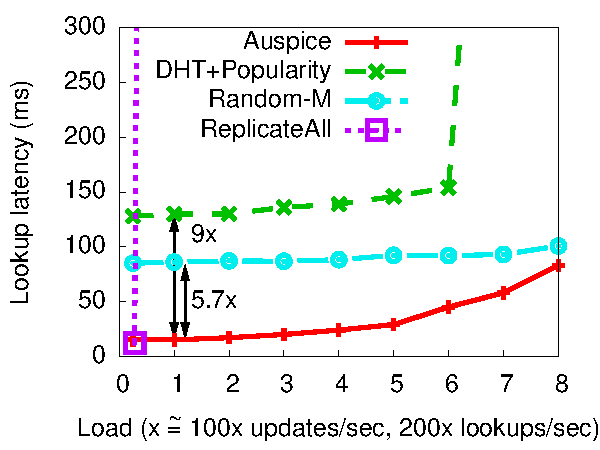
\includegraphics[scale=0.57]{auspice/graph/newgraphs/load-latency.pdf}}
%
%\subfigure[Update cost]{\label{fig:loadupdatecost}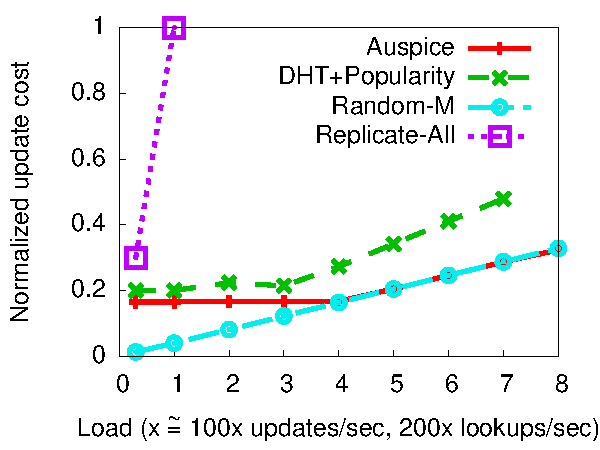
\includegraphics[scale=0.57]{auspice/graph/newgraphs/load-updatecost.pdf}}
%
%\caption{[Cluster] \auspice\ shows 2.2$\times$ to $9\times$ lower latencies over \staticthree\ and \codons\ over a wide rage of loads (0.3 - 6).  \auspice\ can sustain 23$\times$ higher loads than  \replicateall\ due to its lower update costs.}
%\vspace{-0.15in}
%\end{figure}

% and is comparable to the highest loads sustained by other schemes.

%\begin{figure}[ht]
%\centering
%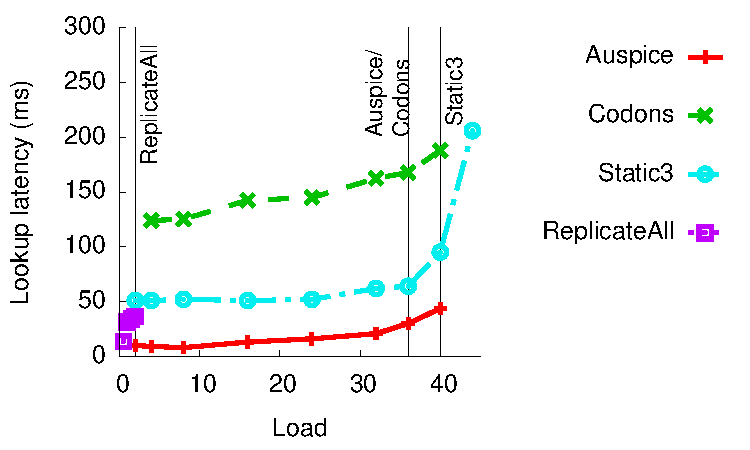
\includegraphics[scale=0.57]{auspice/graph/system-exp/system-load.pdf}
%\vspace{1.5in}
%\vspace{-0.2in}
%\caption{[Cluster] \auspice\ has lower latencies over \staticthree\ and \codons\ over a wide range of loads. Vertical lines show the capacity achieved by  schemes. \auspice\ can sustain 18$\times$ higher loads than \replicateall. TBD: put the load vs. update cost graph here.}
%\label{fig:load}
%\vspace{-0.15in}
%\end{figure}



This experiment analyzes the load-vs-lookup latency behavior of schemes. For every scheme, load is increased  until  2\% of requests (lookups and updates) fail, where a failed request means no response is received until a threshold timeout of 10 sec. Figure \ref{fig:load} shows load-vs-lookup latency curve for schemes; lookup latency metric is the mean of the distribution of median lookup latencies of names. Figure \ref{fig:loadupdatecost} shows the corresponding mean update cost of schemes at varying loads. 

\auspice\ gives 2.2$\times$ to $9\times$ lower latencies over \staticthree\ and \codons\ over a wide range of loads (0.3 - 6). At low to moderate loads, servers have excess capacity than needed sustain the minimum number of replicas for each name. Therefore,  \auspice\ creates as many replicas as possible without exceeding the predetermined threshold utilization level (refer to Equation \ref{eq:mu}). As a result, \auspice\ achieves very small latencies for loads $\leq$ 4. 
At load $\geq$ 4, servers exceed the predetermined threshold utilization level even if \auspice\ creates the minimum number of replicas needed to meet the availability objective. In this regime, \auspice\ only creates only three replicas for each name. This explains why \auspice\ and \staticthree\ have equal update costs for loads $\geq$ 4 (Figure \ref{fig:loadupdatecost}). Reducing the number of replicas at higher loads allows \auspice\ to limit the update cost and sustain a maximum request load that is equal to \staticthree.

%\auspice\ sets a positive value of the replication control parameter ($\beta$) , which results in the creation of more replicas and small lookup latencies. 
% up to $9\times$ lower lookup latency than other schemes. 

\replicateall\ generates a very high update cost and can sustain a request load of at most 0.3. This is further supported by  Figure \ref{fig:loadupdatecost} which shows that the update cost for \replicateall\ at load = 0.4 is more than the update cost of \auspice\  at load = 8.

\codons\  saturates available capacity at a lower load than \auspice\ because of its higher update costs.  
Even though both schemes create nearly equal number of replicas at every load level, \codons\ decides the number of replicas of a name only based on its popularity, i.e., lookup rates, while \auspice\ decides the number of replicas based on lookup-to-update ratio of names. Hence, \codons\  incurs more update costs than \auspice\  due to popular names that also have a high update rate.

}


%\codons\ has higher update costs than \auspice\ and hence saturates available capacity at a lower load. \codons\ has higher update costs than \auspice\ even though both schemes create nearly equal number of replicas at every load level. This is because \codons\ decides number of replicas of a name only based on its popularity, i.e., lookup rates, while \auspice\ decides number of replicas based on lookup-to-update ratio of names. Hence, \codons\  incurs more update costs than \auspice\  due to popular names that also have a high update rate.

%\replicateall\ saturates capacity at a load of 0.3, which is $20\times$  smaller than the maximum sustainable load of all other schemes. This is on account of its high update cost.
%Up to a load value of 4, \auspice\ update cost remains nearly unchanged (Figure \ref{fig:loadupdatecost}, because it chooses a value of  $\beta$ which pushes the update cost to the desired 
 

%This is because it decides the replication control parameter $\beta$ based on request and available. 





%(2) \auspice\ provides smaller lookup latencies than other schemes. due to its cost aware replication enabling it to match \staticthree\ in terms of capacity. \staticthree\ does better as it has a more even distribution of load across name servers.
%
%(3) \codons's replication does not take into account the update costs of names due to which it results in somewhat smaller capacity than other schemes.

% than \auspice\ (Table \ref{tab:fairness}).

%



\eat{This experiment quantifies the performance gap between \auspice\ and the \optimal\ scheme. 
We use simulations for this analysis because \optimal\ is implemented only in our simulator. 
In Figure \ref{fig:optimal}, we present the load-vs-lookup latency curve from this experiment. 
The latency for \auspice\ is between   is 1.14$\times$-2.12$\times$ of the \optimal\ scheme. 
The \optimal\  scheme performs better because it can globally optimize server resource allocation across all names, but \auspice\ uses a decentralized mapping algorithm to independently decide resolver placement for each name. Further, the mapping algorithm in \auspice\ is a simple heuristic, which is sub-optimal. }


\eat{
\begin{figure}[ht]
\centering
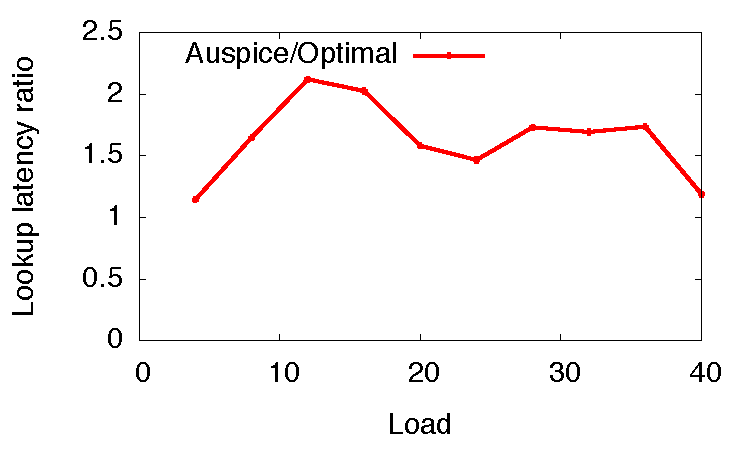
\includegraphics[scale=0.55]{auspice/graph/system-exp/optimal.pdf}
\vspace{-0.1in}
\caption{[Simulator] \auspice's  latency is between 1.14$\times$ and 2.12$\times$  of \optimal.}
\label{fig:optimal}
\vspace{-0.1in}
\end{figure}
}

\eat{
\begin{figure*}[t]
\begin{minipage}[b]{0.3\linewidth}
\centering
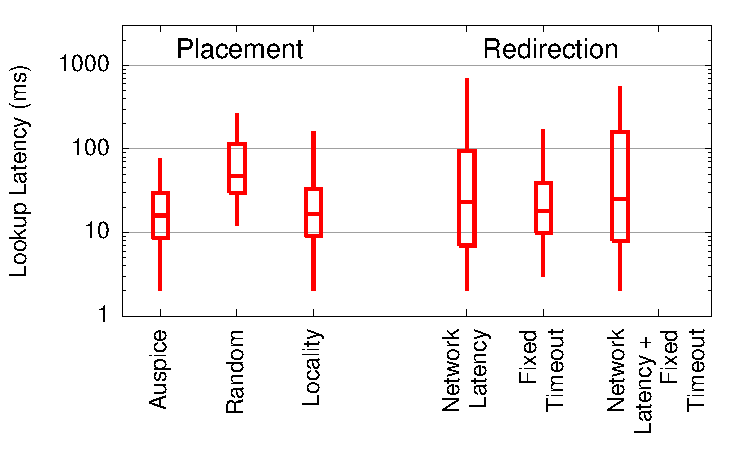
\includegraphics[scale=0.45]{auspice/graph/system-exp/mb-stats.pdf}
\caption{Analysis of \auspice\  shows that a locality-aware placement and redirection based on network and server latency is key to achieve good performance.}
\label{fig:micro}
\end{minipage}
\hspace{0.5cm}
\begin{minipage}[b]{0.3\linewidth}
\centering
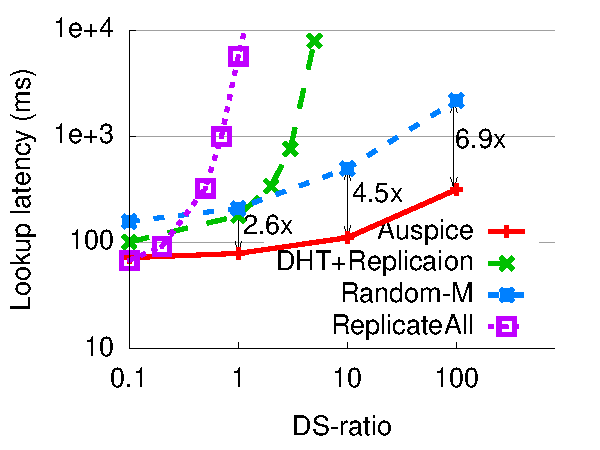
\includegraphics[scale=0.4]{auspice/graph/medianlatencyVSnummobile.pdf}
\caption{[Simulator] \auspice\ scales well to growing number of names and has higher latency gains with more device names.}
\label{fig:varymobile}
\end{minipage}
\hspace{0.5cm}
\begin{minipage}[b]{0.3\linewidth}
\centering
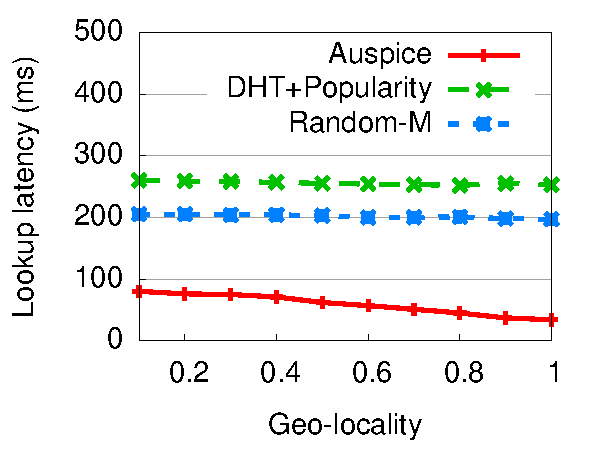
\includegraphics[scale=0.4]{auspice/graph/medianlatencyVSlocality.pdf}
\caption{[Simulator] \auspice\ outperforms other schemes by 2$\times$ to 5$\times$  across all locality levels. \replicateall\ has X\% failure rate of requests.}
\label{fig:varylocality}
\end{minipage}
\vspace{-0.15in}
\end{figure*}
}
\vsp
\subsubsection{Update propagation latency}
\label{sec:updatelatency}


\begin{figure*}[ht]
\vspace{0.05in}
\begin{minipage}[b]{0.3\linewidth}
\centering
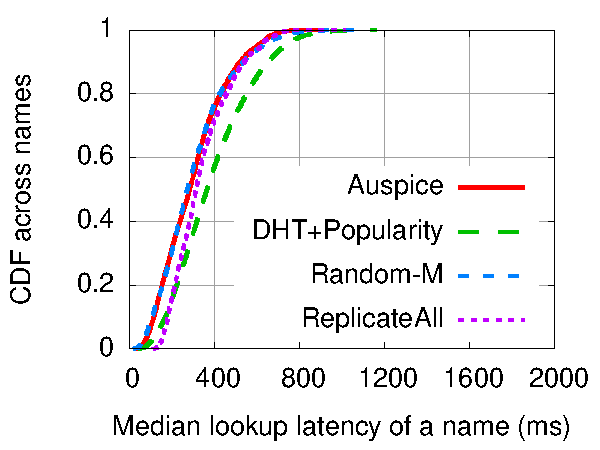
\includegraphics[scale=0.55]{auspice/graph/newgraphs/update-latency-cdf.pdf}
\caption{[System] Median update latency of \auspice\ is 284ms and is comparable to other schemes.} 
\label{fig:updates}
\end{minipage}
\hspace{0.3cm}
\begin{minipage}[b]{0.35\linewidth}
\centering
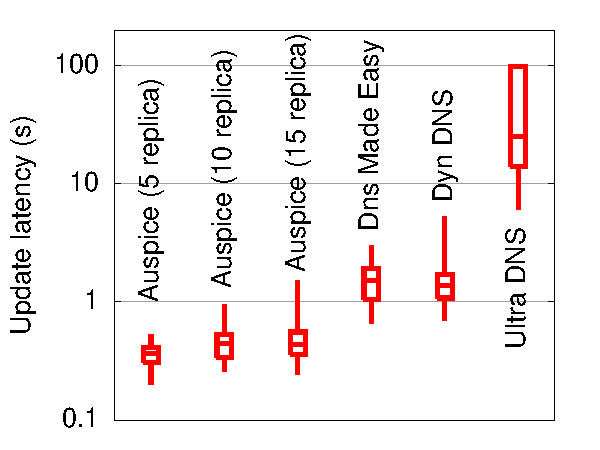
\includegraphics[scale=0.55]{auspice/graph/newgraphs/managed-update.pdf}
\caption{Update propagation latency of \auspice\ for updating replicas at 5 locations is  1.0 sec to 24.7 sec lower than three top-tier managed DNS providers. }
\label{fig:manageddnsupdate}
\end{minipage}
\hspace{0.3cm}
\begin{minipage}[b]{0.3\linewidth}
\centering
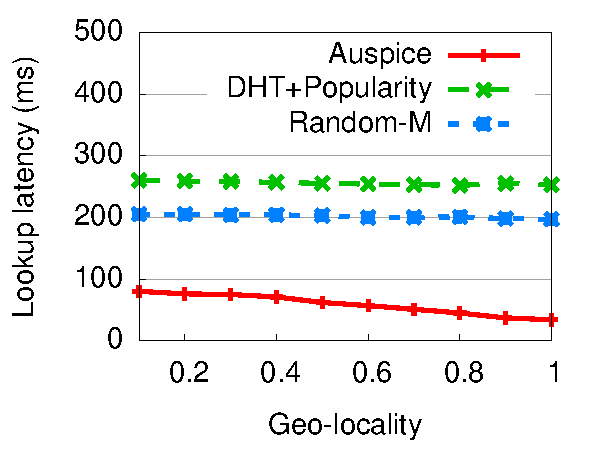
\includegraphics[scale=0.53]{auspice/graph/medianlatencyVSlocality.pdf}
\caption{[Simulator] Workload sensitivity. \auspice\ gives 2$\times$ to 5$\times$  lower latency across locality levels.}
\label{fig:varylocality}
\end{minipage}
%\vspace{-0.25in}
\end{figure*}


\eat{
\begin{figure}[h]
\centering
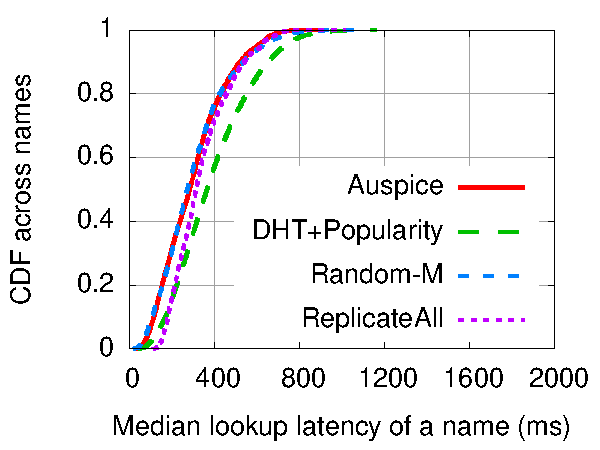
\includegraphics[scale=0.55]{auspice/graph/newgraphs/update-latency-cdf.pdf}
%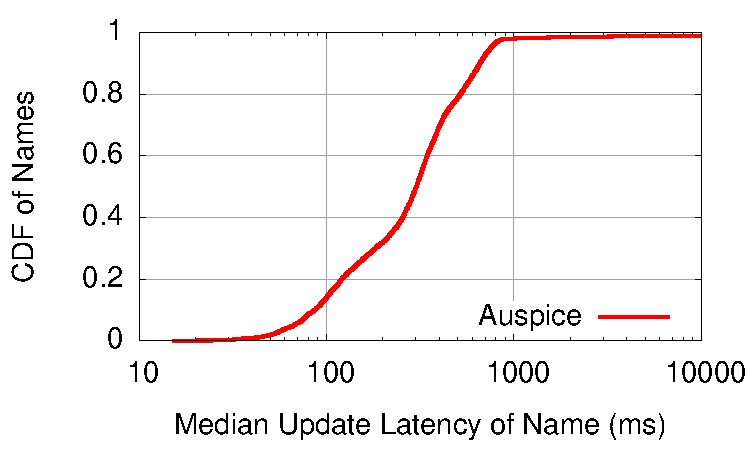
\includegraphics[scale=0.55]{auspice/graph/system-exp/cdf-names-median-update.pdf}
\vspace{-0.2in}
\caption{[System] Median update latency of \auspice\ is 284ms and is comparable to those of other schemes.} 
%The high latencies for \replicateall\ are because of insufficient upload capacity on PlanetLab.}
\label{fig:updates}
\vspace{-0.1in}
\end{figure}


\begin{figure}
\centering
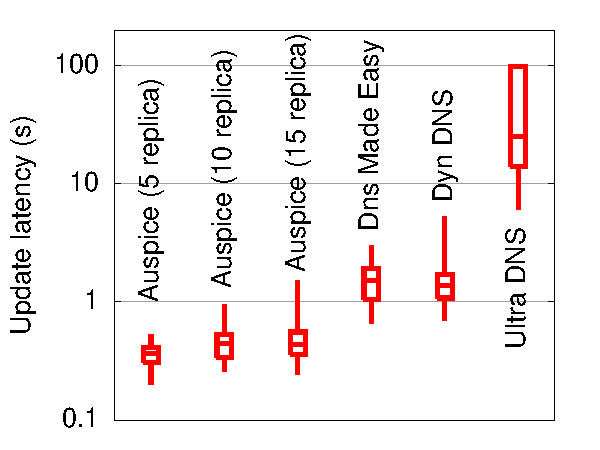
\includegraphics[scale=0.55]{auspice/graph/newgraphs/managed-update.pdf}
\vspace{-0.1in}
\caption{Median  update latency of \auspice\ for updating replicas at 5 locations is  1.0 sec to 24.7 sec lower than three managed DNS providers. Values shown are 5, 25, 50, 75,  and 95 percentiles.}
\vspace{-0.2in}
\label{fig:manageddnsupdate}
\end{figure}


\begin{figure}[t]
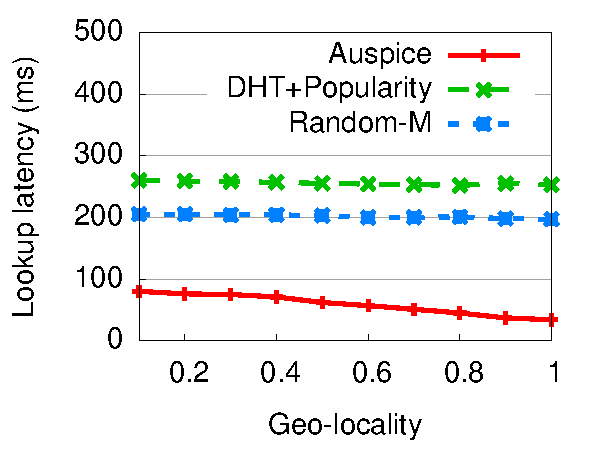
\includegraphics[scale=0.5]{auspice/graph/medianlatencyVSlocality.pdf}
\vspace{-0.1in}
\caption{[Simulator] Workload sensitivity. \auspice\ gives 2$\times$ to 5$\times$  lower latencies across all locality levels.}
\label{fig:varylocality}
\vspace{-0.1in}
\end{figure}

}
%\subfigure{\label{fig:updatelatency}\includegraphics[scale=0.55]{auspice/graph/newgraphs/}}

%This experiment evaluates the update latency of schemes.

The time-to-connect latency is determined primarily by the lookup latency and the {\em update propagation latency} (refer Fig. \ref{fig:4mobility}), i.e., the time from when a client issued a write till the last replica executes the write. With eventual consistency, update propagation takes one round, while with total write ordering, update propagation takes two rounds and twice the messages.

Figure \ref{fig:updates} shows the distribution of the median {\em client-perceived update latencies}, i.e., the time from when when a client sends an update to when it receives confirmation, with total write ordering.  These numbers are from the experiment in Section  \ref{sec:lowload} for load = 0.3. The median and 90th percentile update latency for \auspice\ is 284 ms and is comparable to other schemes. A request, after arriving an active replica, takes four one-way network delays to be committed by Paxos, which explains why update latency of all schemes is a few hundred ms. 

Next, we measure the update propagation latency. With lazy propagation, this time is 154 ms, while with total write ordering, this time is 292ms. Thus. the cost of the stronger consistency provided by total write ordering compared to lazy propagation is that it can increase the time-to-connect latency by up to 2$\times$, which is as expected. Note however, that the 2$\times$ inflation is a worst-case estimate, i.e., it will impact the time-to-connect latency only if a read request arrives at a replica while a write is under propagation to that replica.

%Paxos'  consistency guarantees come at the cost of increased update latencies. We quantify how much update latencies could be reduced with the following update protocol, called \emph{lazy-update},  which gives eventual consistency:  send confirmation to client after updating locally, and then propagate the update to other replicas. A client would get a confirmation sooner in case of lazy-update, but the update might take longer to be actually received by all replicas. In another experiment, we measured the  time  lazy-update takes to propagate the update to all replicas. We measure the median of the distribution of time to update all replicas to be 154 ms for lazy-update. The corresponding median values for Paxos is 292ms. Thus, Paxos increases the  latency to propagate updates to all replicas by  1.8$\times$ over eventual-consistency.
% We  measured update latency as time difference between when a client sends and update and when the update gets committed at all active replicas. 


%We calculate the time lazy-update would take to propagate an update to all replicas. 
%For every update, we calculate the time lazy-update would take to propagate an update to all replicas
%, based on offline analysis of the workload 
%
%For all replicas to be updated, lazy-update would 
%
% Such a protocol, would return a confirmation to client after updating locally, and would then propagate the update to other replicas. 
%
%For every update, 

%What would the latencies for \auspice\ be if all updates were not executed in the order they were committed 



%Figure \ref{fig:updates} shows the distribution of median update latencies from the the experiment in Section  \ref{sec:lowload} for load = 0.3. The median and 90th percentile update latency for \auspice\ is 284 ms and 522 ms respectively. A request, after arriving an active replica, takes four one-way network delays to be committed by Paxos, which explains why update latency of all schemes is a few hundred ms.
%As described in Section \ref{sec:consistency}, an address update takes six wide-area network delays  including the delay from client to the nearest active replica, which explains why update latency of all schemes is a few hundred ms. 

%\codons\ has higher update latency because the delay from the client to the active replica that receives the update request is higher for \codons\ compared to other schemes; \codons\ selects this active replica using consistent hashing while other schemes select the nearest available active replica. Note that if the schemes used write-to-one with lazy update propagation instead of Paxos, their update latencies would be much smaller like the lookup latencies in Figure \ref{fig:lookupupdate}(a).
%\tbd{Check this claim}.

%\vsp
%\subsubsection{[Simulation] Comparison to \optimal}
%\label{sec:optimal}




%How does update latency affect clients? A lookup request for a name while its address update is in progress may return an incorrect response to a client. An update latency of few hundred milliseconds implies that a client who receives an incorrect response will be able to lookup correct addresses for the name on retrying after a few hundred milliseconds.


%\codons\ 
%
%\staticthree\ and \codons\  have nearly the same update latency as \auspice, while \replicateall\ has a higher update latency (median = 521 ms).   


%Since the update latency is a few hundred ms, the client can lookup the correct addresses on retrying at most few hundred ms. 
% This interval is typically a few hundred ms as shown by this experiment. However, the client can lookup the correct addresses on retrying once the update is complete.






%and are comparable to that of \staticthree\ and \codons.  \replicateall\ has the highest update latencies  as it propagates updates to a much greater number of replicas.  The \replicateall\ scheme has median update latencies of 100-1000 seconds for 15\% of names. This is because updates for these names are handled by nodes whose upload capacity is less than that required by \replicateall. Hence, updates get queued at name sever and completed updates have high update latencies. 


%Update latency for \auspice\ is a few hundred milliseconds due to our Paxos implementation. An address update is first sent to the Paxos co-ordinator for this name record,  which waits for a confirmation from a majority of replicas, and then replies to the client that the update is complete.  Since the Paxos co-ordinator is chosen randomly among replicas, update latency for \auspice\ is roughly equal to twice of the RTT between a pair of randomly chosen PlanetLab nodes. 

%\begin{figure}
%\centering
%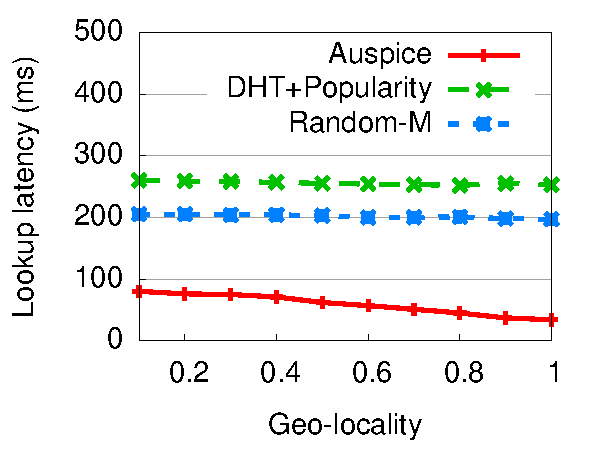
\includegraphics[scale=0.5]{auspice/graph/medianlatencyVSlocality.pdf}
%\vspace{-0.1in}
%\caption{[Simulator] \auspice\ outperforms other schemes by 2$\times$ to 5$\times$  across all locality levels. \replicateall\ has nearly 100\% failure rate of requests (not shown).}
%\label{fig:varylocality}
%\vspace{-0.1in}
%\end{figure}





%The frequency of lookups for device names is difficult to predict and will depend on how applications are designed in future. For example, if push-based applications are popular, we expect more frequent lookups for device names. This experiment evaluates performance for different lookup rates of device names. Experiment to be done.


%\begin{figure}[t]
%\centering
%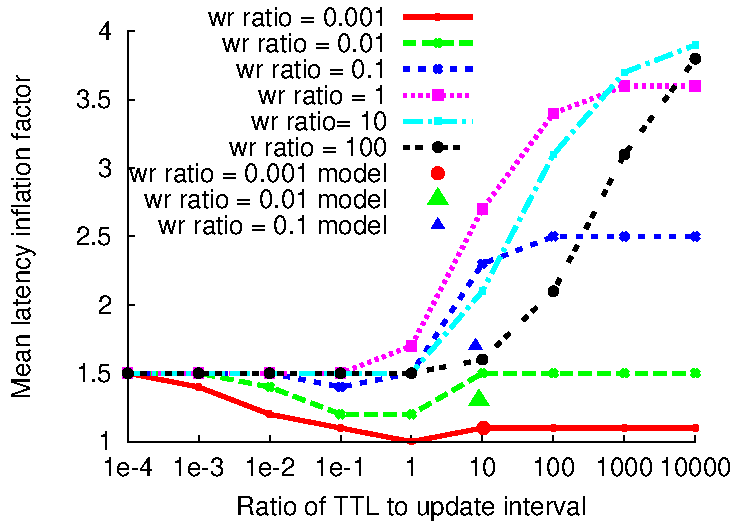
\includegraphics[scale=0.5]{auspice/graph/meanlatencyinflationfactor.pdf}
%\vspace{-0.1in}
%\caption{[Simulator] Mean latency inflation factor as a function of TTL.}
%\label{fig:meanlatencyinflationfactor}
%\vspace{-0.1in}
%\end{figure}

%\begin{figure}[t]
%\centering
%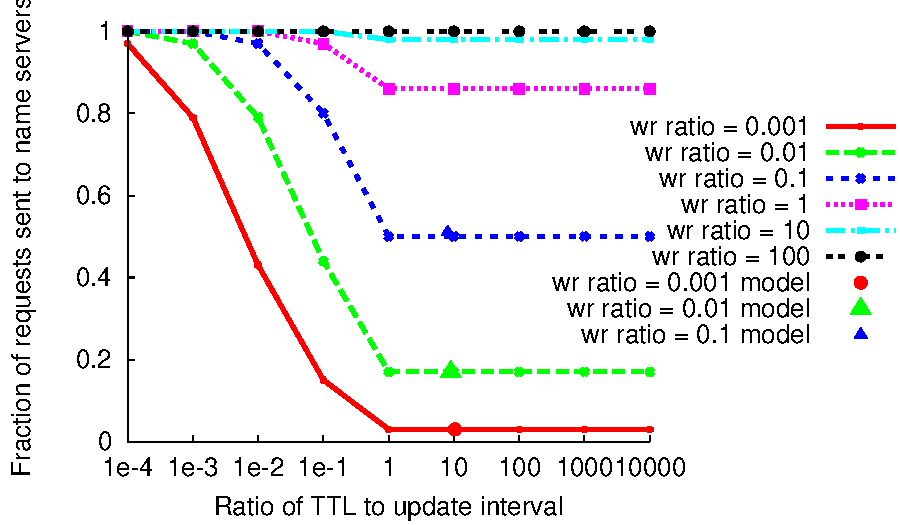
\includegraphics[scale=0.5]{auspice/graph/fractionrequest.pdf}
%\vspace{-0.1in}
%\caption{[Simulator] Fraction of requests that are sent to the name servers.}
%\label{fig:fractionrequest}
%\vspace{-0.1in}
%\end{figure}







%This experiment shows that \auspice\ provides smaller update latencies than commercial managed DNS providers. 

%\auspice\ provides a median update improvement  latency of 0.31 s, while the three providers have median update latencies of 662 ms, 1396 ms and 25 sec respectively. It's not clear  why ``Managed DNS 3" update latencies are an order of magnitude higher than global propagation delays.  Another recent study  has also shown that multiple managed DNS providers have update latencies of up to tens of seconds \cite{dnscompare}. This experiment shows that \auspice\ provides smaller update latencies than commercial managed DNS providers. 





\eat{

\begin{figure*}[t]
\begin{minipage}[b]{0.3\linewidth}
\centering
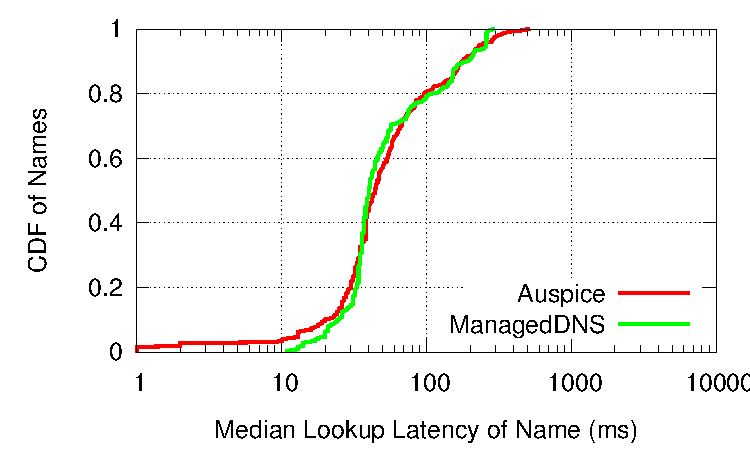
\includegraphics[scale=0.45]{auspice/graph/system-exp/dns-names.pdf}
\caption{\auspice\ has median latencies comparable  to managed DNS provider by placing only 5 resolvers in a locality-aware manner.}
\label{fig:manageddns}
\end{minipage}
\hspace{0.5cm}
\begin{minipage}[b]{0.3\linewidth}
\centering
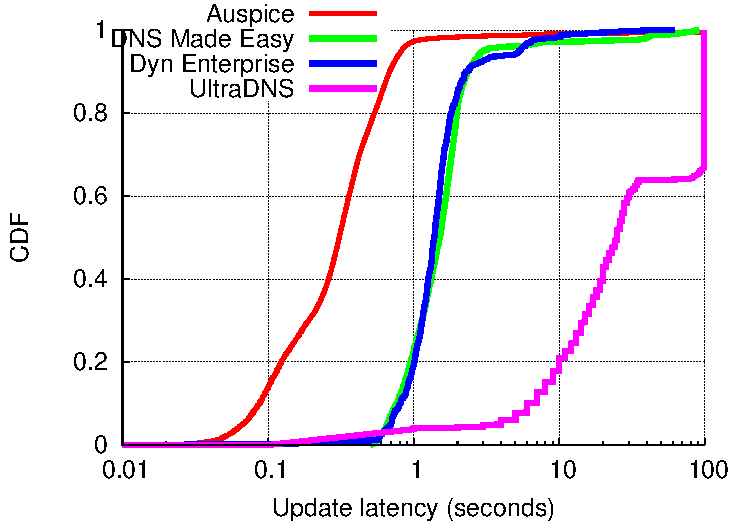
\includegraphics[scale=0.45]{auspice/graph/updatelatencycdf.pdf}
\caption{The  median  update latency of \auspice\ is  354 ms, 1.08 sec, and 24.7 sec lower than three managed DNS providers.}
\label{fig:manageddnsupdate}
\end{minipage}
\hspace{0.5cm}
\vspace{-0.15in}
\end{figure*}

}

\eat{
\vsp
\subsection{Mid-session mobility}
\label{sec:mobility}

\begin{figure}[ht]
\centering
\vspace{-0.1in}
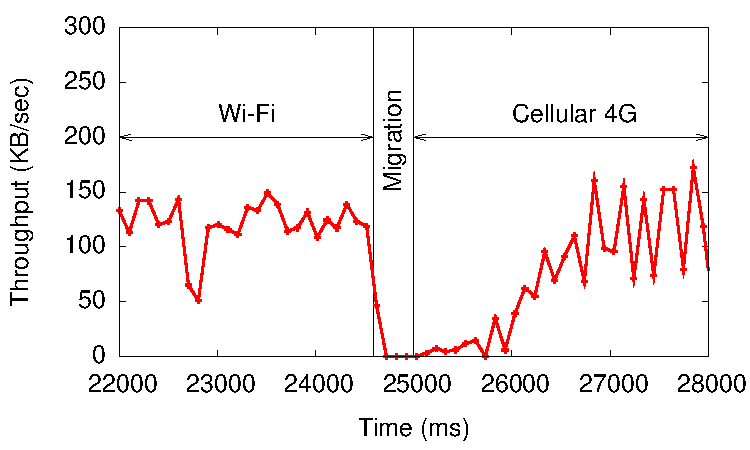
\includegraphics[scale=0.55]{auspice/graph/system-exp/Plot.pdf}
\vspace{-0.1in}
\caption{Client throughput  during a migration from Wi-Fi to 4G. Migration period is from 24585 ms to 24997 ms.}
\label{fig:mobility}
\vspace{-0.1in}
\end{figure}

This experiment demonstrates a connection end-point migration across networks using the MSocket library; migration involves a bilateral negotiation between client and server. 
Figure \ref{fig:mobility} shows the client's throughput during  the experiment. 
Each point is the average TCP throughput within last 100 ms. 
At t = 0, the client, which a laptop equipped with Verizon 4G USB modem,  uses a Wi-Fi  connection to start a large file transfer from a server. At t = 24585 ms, the client calls the \verb+migrate_local()+ function  to switch to a 4G connection. 
The function call returns after 412 ms confirming a successful migration. 
In Figure \ref{fig:mobility}, connection throughput drops to zero during the migration period and increases once the migration is complete.
The migration takes nearly three round trip times as the average RTT between the client and the server over a 4G connection is 140 ms.
In the first RTT, client sends a SYN packet and the server responds with a SYN/ACK packet.  In the second (third) RTT,  the client (server) sends a control message  containing its MSocket flow ID and sequence number,  and the server (client) responds with an ACK. 
}



